%% Capitolul 0: INTRODUCERE
%%
%%

\addcontentsline{toc}{chapter}{Introducere}
\markboth{\bf Introducere}{\bf Introducere}

\chapter*{Introducere}
\label{capintro}
\markboth{\bf Introducere}{\bf Introducere}

@Inv@a@tarea automat@a a devenit un subiect de interes din ce @in ce mai important, aceast@a fiind utilizat@a @in vaste domenii, precum: industria auto, alimentar@a, agricol@a, bancar@a, aerospa@tial@a @si mai cu seam@a @in industria tehnologiei informa@tiei. Unul din rolurile ei cele mai importante const@a @in analiza @si clasificarea datelor, predic@tia unor evenimente @in baza unor fapte deja @int@amplate, crearea unui profil virtual pentru un grup de utilizatori, etc.


Datorit@a marei conectivit@a@ti dintre oamenii din ziua de ast@azi; sistemele politice, economice @si rela@tiile interumane au devenit extrem de complexe. Totul a devenit interconectat. O ideea a unui singur individ poate fi transmis@a pe tot globul p@am@antesc, aceasta idee putand afect\^ and milioane de oameni \^ in diverse locuri @si a c\^ arui impact politic @si economic poate fi greu de estimat. De asemenea, un incident economic local, un dezastru natural, sau un conflic politic dintre dou@a @t@ari pot avea efecte devastatoare asupra economiei globale @si a structurii geopolitice curente.

Fiecare eveniment din ziua de ast@azi are o influen@t@a mai mic@a sau mai mare aupra acestei mari re@tele de sisteme ale civiliza@tiei umane. @Intrebarea natural@a la aceast@a dilemna este: putem face o estimare aupra acestor evenimente @si ale cazurilor lor speciale? Se poate, @si asta datorit@a faptului ca multe evenimente sunt monitorizate @si @inregistrate, precum: tranzac@tiile bancare, documente legislative @si juridice, vremea, traseele @si destina@tiile ma@sin@ariilor de transport marf@a (automobile, avioane, vapoare), discursuri @si opinii @in re@tele sociale, date medicale din dispozitive inteligente (telefoane smart, ceasuri @si br@atari smart), date provenite din simul@ari virtuale sau experimente. 

Tot acest mare volum de informa@tii @si metodele de manipulare, stocare @intr@a @in a@sa numita categorie {\sl Big Data}. Analiz@a acestui volum imens de date devine o sarcin@a foarte dificil@a @si laborioas@a @in cazul metodelor conven@tionale de analiz@a a datelor folosind statistic@a clasic@a. @In esen@t@a, @inv@a@tarea automat@a se foloseste at@at de teoria clasic@a c\^  at @si de noile descoperiri @in calculul numeric pentru a crea modele matematice dinamice care pot acumula cuno@tin@te @si ac@tiona @in baza lor folosind toate datele pe care le prime@ste ca set de @inv@a@tare.


\^ In aceast\u a lucrare se va analiza cum algoritmii de @inv@a@tare automat@a  pot fi folosi@ti @in crearea unui agent autonom care s@a @indeplineasc@a sarcinii @intr-un spa@tiu 2-dimensional. Problema va consta @in crearea unui mediu 2-dimensional @in care un agent trebuie s@a ghideze o ma@sin@a astfel @inc\^ at aceast@a s@a parcurg@a cu succes un traseu.
\hspace{0.2cm}

\^ In primul capitol este descris termenul de @inv@a@tare automat@a, care sunt subdomeniile sale, cum este folosit @in @industire. @In al doilea capitol este o mic@a introducere pentru re@telele neuronale artificiale.

\^ In al treilea capitol vor fi prezenta@ti c@a@tiva algoritmi de @inv@a@tare, iar al patrulea descrierea aplica@tiei.

\newpage

%%CAPITOLUL 1
%%
%%
\chapter{ @Inv@a@tare automat@a }
\index{capitol!C1}

\section{Istoric}
\index{sectiune!S1.1}

	@Inv@a@tarea automat@a este o ramur@a a @inteligen@tei artificiale care se ocup@a cu studiul tehnicilor @si metodelor prin care se ofer@a unui calculator abilitatea de a @inv@a@ta. Prin @inv@a@tare ne referim la posibilitatea de a oferii o decizie @in baza unor cuno@stin@te deduse din experien@te anterioare.

 Multe tehnici din @inv@a@tarea automat@a au la baz@a modelul de interac@tiune al neuronilor, descris de c@atre Donal Hebb @in cartea sa {\sl The Organization of Behavior} \cite{donald-hebb-book}. Termenul de @inv@a@tare automat@a (@in englez@a {\sl machine learning}) a aparut @in anul 1953, dat de Arthur Samuel, creatorul unui program de jucat checker, capabil s@a ia decizii bazate pe experien@tele anterioare \cite{arthur-samuel}. @In anul 1957, Frank Rosenblatt creaz@a Perceptron-ul - utilizat @in crearea unui calculatorul capabil s@a recunoasc@a forme @intr-o imagine - folosindu-se de observa@tiile din lucr@arile lui Donald Hebb @si Arthur Samuel. Perceptron-ul de unul singur are o putere destul de limitat@a, dar odat@a cu descoperirea utiliz@arii sale @in combina@tii de mai multe straturi a dat na@stere la termenul de re@tea neuronal@a. 
 
 De-a lungul timpului, acest domeniu a avut o evolu@tie @inceat@a, un factor important find capabilit@a@tile limitate de procesarea ale calculatoarelor. Dar odat@a cu avansurile tehnologice, cercetarea @in acest domeniu a @inceput s@a fie din ce @in ce mai activ@a, @in ultimii ani culmin\^ and cu evenimente care au atras interesului publicului general, precum: IBM's Deep Blue, IBM's Watson, Google's Deepmind @si Google's AlphaGo.
 
 
\newpage

\section{Clasificare}

Fiind un domeniu foarte vast @si cuprinz@tor, aceasta se @imparte @in 3 mari categorii:
\hspace{0.2cm}\begin{itemize}
	\item @Inv@a@tare supervizat@a
	\item @Inv@a@tare nesupervizat@a
	\item @Inv@a@tare prin recompens@a
\end{itemize}

\vspace{0.3cm}
@In @inv@a@tarea supervizat@a, procesul de antrenare se bazeaz@a pe analiza unor date formate din perechi de valori intrare-ie@sire (set de date etichetat) pentru calibrarea func@tiilor de deducere. Este folosit pentru rezolvarea problemelor de clasificare.

Exemple de algoritmi:
\begin{itemize}
	\item Support-vector machines
	\item Regresia liniar@a
	\item Regresia logistic@a
	\item Arbori de decizie
	\item Re@tele neuronale
	\item Clasificator bayesian naiv
\end{itemize}

Pentru @inv@atarea nesupervizat@a, procesul de antrenare const@a @in crearea unor modele interne de recunoa@stere a unor tipare @in urma analizei unui set de date neetichetat. Este deseori folosit @in descoperirea similarit@a@tilor @si diferen@telor @intr-un set de date.

Exemple de algoritmi:
\begin{itemize}
	\item K-means clustering
	\item Autoencoders
	\item Analiza componentei principale
	\item Descompunerea valorilor singulare
\end{itemize}

@In @inv@a@tarea prin recompens@a, procesul de antrenare const@a @in maximizarea unei func@tii de recompens@a, modelul calibr@andu-se astfel @incat deciziile luate s@a duc@a spre ob@tinerea unei recompense c\^ at mai mari.

Exemple de algoritmi:
\begin{itemize}
	\item Monte Carlo
	\item Q-learning
	\item SARSA
	\item Deep Q Network
	\item Proximal Policy Optimization
	\item Deep Deterministic Policy Gradient
	\item Trust Region Policy Optimization
\end{itemize}

\section{Industrie}

	Tot mai multe aplica@tii folosesc tehnici de @inv@a@tare automat@a pentru optimizarea produselor, servicilor @si interac@tiunilor cu utilizatorii. Cele mai notabile utiliz@ari fiind:
\begin{itemize}
	\item Algoritimi de c@autare a @stirilor @in baza unor preferin@te oferite explicit sau implicit de catre utilizator.
	\item Reclame personalizate generate dup@a profilele utilizatorilor.
	\item Sisteme de recomand@ari produse.
	\item Etichetarea obiectelor sau persoanelor @in imagini, @inregistr@ari audio sau video.
	\item Sisteme robotice autonome.
	\item Ma@sini autonome.
	\item Sisteme meteorologice
	\item Sisteme de detectare a fraudelor @intr-un sistem bancar.
	\item Clasificare @si predic@tia evenimentelor. 
	\item Optimizarea proceselor de produc@tie a m@arfurilor.
	\item Optimizarea procesului de antrenare pentru atle@ti.
\end{itemize}

	Companiile sunt foarte interesate de modul cum interac@tioneaz@a @si percep clien@tii produselor lor, ele @incerc\^ and mereu s@a colecteze informa@tii pentru despre modul cum sunt utilizate produsele @in activitatea utilizatorului. Aceste campanii de colectare a datelor a devenit din ce @in ce mai agresiv@a, marile companii software specializate @in re@tele sociale (Facebook, Twitter, Youtube, Linkedin, Reddit) v@and datele utilizatorilor @in vederea oferirii unui profil al consumatorului pentru a stabili interesul pentru produs. 
	 
\section{Programe software pentru dezvoltare}

Interesul puternic pentru acest domeniu a venit @in principal din partea marilor companii software @si hardware, ele dezvolt@and puternice biblioteci pentru procesarea datelor, crearea de re@tele neuronale, algoritmi de @inv@a@tare, etc. Pentru sprijinirea domeniului, aceste unelte sunt oferite dupa ca aplica@tii cu surs@a deschis@a ( @in englez@a {\sl open source} ), av@and o licen@t@a deseori foarte permisibil@a @in vederea utiliz@ari personale @si comerciale.

Calitatea acestor unelte le-a f@acut s@a devin@a un standard @in industrie, at@at comercial@a c\^ at @si academic@a.

Example de biblioteci sau aplica@tii software:

\begin{itemize}
	\item Tensorflow - bibliotec@a dezvoltat@a de c@atre Google @in vederea utiliz@ari cu usurin@t@ a algoritmilor de @inv@a@tare, c@at @si func@tii utilitare pentru manipularea datelor.
	\item PyTorch - bibliotec@a dezvoltat@a de c@atre Facebook pentru protiparea aplica@tilor de viziune computerizate, procesarea limbajului natural, etc.
	\item ML.NET - bibliotec@a dezvoltat@a de Microsoft pentru crearea rapid@a a unor aplica@tii de procesare a datelor folosind algoritmi de @inv@a@tare.
	\item scikit-Learn - bibliotec@a care con@tine func@tii statistice folosite pentru analiza datelor.
	\item Apache Spark - bibliotec@a de aplica@tii destinate pentru procesarea unui volum foarte mare de date.
	\item Apache Kafka - aplica@tie care permite stocarea @si distribuirea unui volum foarte mare de date @in timp real c@atre mai mul@ti consumatori.
	\item Caffe - bibliotec@a pentru dezvoltare aplica@tilor pentru medii de lucru care nu dispun de o putere de procesare foarte mare, precum dispozitivele mobile.
	\item Keras - bibliotec@a pentru dezvoltarea re@telelor neuronale
	\item H2O.ai - platform@a de procesare @si analiz@a a datelor pentru mediul comercial
	
\end{itemize}

\section{Big Data}

O component@a esen@tial@a pentru @inv@a@tarea automat@a este gestionarea datelor care vor fi folosite @si produse de c@atre algoritmi algoritmii @inv@a@tare. Aceast@a gestionare a informa@tiilor, de cele mai multe ori, va intra @in cadrul domeniului de {\sl Big Data }

Conform Uniunii Europene: ,,Big data se refer@a la volume de date colectate at\^ at de mari @si complexe @inc\^ at este nevoie de noi tehnologii, cum ar fi inteligen@t@a artificial@a, pentru a le procesa. Datele provin din nenum@arate surse diferite.''\cite{eu-big-data-definition}

Volumul de date pe care omenirea @il produce cre@ste de la an la an, cea ce face  analiza @si intelegerea datelor s@a fie o sarcin@a din ce @in ce mai dificil@a. Tot mai mul@ti oameni @incep s@a aib@a acces la internet, iar num@arul de dispozitive inteligente (smart phone, smart watch, smarth TV) pe care un individ de dispune cre@ste odat@a cu avansul tehnologic.

Principalele surse de provenien@t@a ale acestor date sunt:
\begin{itemize}
	\item Re@tele sociale - mesaje, imagini create de utilizatori pentru a@si exprima opinia la situa@tia sociala, economic@a @si politic@a - datele pot fi utilizate pentru stabilirea unor tendin@te sociale cu privire la activitatea @si starea emo@tional@a curent@a @si viitoare a oamenilor.
	\item Mediul @si natura - date provenite de la sateli@ti @si senzori pentru monitorizarea schimb@arilor climatice - folosite pentru predic@tia posibilelor dezastre naturale cauzate de activit@a@tile omului.
	\item Sector public - documente, certificate, atestate, adeverin@te emise de c@atre institu@tile publice - pot fi utilizate @in eficientizarea servicilor publice.
	\item Transport - date colectate prin GPS @si de la diferi@ti operatori @in domeniul transportului (transportul public, aeroporturi, g@ari) - pentru optimizarea rutelor @si a curselor de transport.
	\item Sector Medical - fi@se medicale ale pacien@tilor - monitorizarea st@arii de s@anatatea a cet@a@teinolor, utile pentru detectarea posibilelor amen@t@ari de tip biologic.
	\item Iternetul Lucrurilor ({\sl Internet of Things}) - date provenite de la diverse aparate, precum: telefon, ceas, televizor, senzor de gaz, sensor de umiditate, camere video, etc. - utilizate la monitorizare activit@a@tii invidului cu scopul de a u@sura anumite sarcini sau pentru a prevenii incidente.
	\item Sector industrial - re@tele industriale de comunica@tii ( senzori, magistrale de teren, re@tele celulare), rapoarte economice - folosite pentru automatizare @si @imbun@at@a@tirea produselor @si a servicilor. 
	\item Sector bancar - tranzac@tii financiare, rapoarte - utilizate pentru detectarea fraudelor bancare, stabilirea ratelor la dob@anzi, @imprumuturi, schimb valutar, etc.
\end{itemize}

Toate aceste benificii sunt importante pentru societatea din ziua de ast@azi, companii mare concureaza pentru crearea de infrastructur@a @si servicii pentru stocarea @si examinarea datelor.

Exemple de servicii:

\begin{itemize}
	\item Amazon Web Services - cel mai mare furnizor de servicii @si infrastructur@a cloud din lume (av\^ and peste 200 de solu@tii software).
	\item Microsoft Azure 
	\item Google Cloud Platform
	\item IBM Cloud
	\item Oracle Cloud
	\item Alibaba Cloud
\end{itemize}

	
%%CAPITOLUL 2
%%
%%

\chapter{Re@tele neuronale artificiale}

\index{capitol!C2}

\section{Introducere}

O re@tea neuronal@a artificial@a este un model computa@tional inspirat din structura @si modul de fun@tionare al creierului biologic. Conexiunile dintre neuronii artificiali se asem\^ an@a sinapselor, fiecare neuron se conecteaz@a cu alt neuron prin intermediul unor muchii. Semnalul trimis prin aceste muchii este ponderat de ni@ste parametri numi@ti ponderi sinaptice. Mai mul@ti neuroni grupa@ti formeaza un strat, iar mai multe straturi formeaz@a o re@tea.

Procesul de @inv@a@tare presupune g@asirea unor valori potrivite pentru ponderile sinaptice astfel @inc\^ at procesarea semnalului de intrare s@a ofere rezultatul dorit.


\section{Structur@a}

Structura principal@a al unui neuron artificial este bazat pe modelul Perceptron-ului al lui Donald Hebb, modelul matematic fiind:

$$
	y = \varphi \left( \sum_{k=1}^{n} w_k * x_k + b \right)
$$

,unde $x$ este vectorul de intrare, $y$ vectorul de ie@sire, $w$ ponderea sinaptic@a, $b$ deplasarea @si $\varphi$ este func@tia de activare.

Vectorul de intrare este format din numerele reale, aceste numere put\^ and reprezenta: imagini, frecven@te, etichete codificate, valori provenite din senzori, etc. Ponderile sinaptice au rolul de a cre@ste sau descreste puterea semnalul reprezentat de valorile vectorului de intrare. Func@tia de activare preia semnalul ponderat @si ofer@a o valoarea spefic@a @in baza acestuia. Deplasarea ajut@a la deplasarea semnalului ponderat pentru o mai bun@a aproximare necesar@a pentru @indeplirea anumitor condi@tii ale func@tiei de activare.

\begin{exemplu}

	Un neuron artificial care ac@tioneaz@a precum o poarta logic@a {\bf SAU}(OR) pentru dou@a numere binare are forma:
$$
	y = \varphi ( x_1 + x_2 - 0.5 )
$$
,unde $x = \{ x_i | x_i \in \{0, 1\} \}$, $y \in \{0, 1\}$, $w_1 = 1$, $w_2 = 1$,$b = -0.5$, iar func@tia de activare este: 
$$
	\varphi ( u ) = \left\lbrace
		\begin{array}{lc}
			1 & u \geq 0 \\
			0 & u < 0
		\end{array}
	\right.
$$
\end{exemplu}

{\bf Verificare}. Pentru $x = [1, 0]$, avem $u = 1 + 0 - 0.5 = 0.5$ @si $y = \varphi(u) = \varphi(0.5) = 1$ (acela@si rezultat @si pentru $x = [0, 1]$ - datorit@a propieta@tii de comutativitate a adun@arii).
Pentru $x = [1, 1]$, avem $u = 1 + 1 - 0.5 = 1.5$ cu $\varphi (u) = \varphi ( 2 ) = 1$. Ultimul caz pentru $x = [0, 0]$, vom avea $u = $

\begin{observatia}
	F@ar@a func@tia de activare, perceptronul ac@tioneaz@a precum o func@tie liniar@a. Prin utilizarea unei func@tii de activare potrivite, puteam aborda mai u@sor problemele neliniare, precum cele pentru clasificarea datelor @in diverse categorii.
\end{observatia}

Un singur perceptron ofer@a doar o singur@a valoare de ie@sire. Dac@a dorim s@a avem mai multe valori de ie@siri trebuie s@a mai adaug@am perceptroni. Gruparea de neuroni artificiali se nume@ste {\sl strat}.

Structura unui strat arat@a astfel @in form@a matriceal@a:

$$
	\begin{bmatrix}
		u_1 \\
		u_2 \\
		\vdots \\ 
		u_n \\
	\end{bmatrix}	
	= 
	\begin{bmatrix}
		w_{11} & w_{12} & \cdots & w_{1n} \\
		w_{21} & w_{22} & \cdots & w_{2n} \\
		\cdots & \cdots & \cdots & \cdots \\
		w_{n1} & w_{n2} & \cdots & w_{nn} \\
	\end{bmatrix}
	\begin{bmatrix}
		x_1 \\
		x_2 \\
		\vdots \\
		x_n \\
	\end{bmatrix}
	+
	\begin{bmatrix}
		b_1 \\
		b_2 \\
		\vdots \\
		b_n
	\end{bmatrix}
$$

$$
\begin{bmatrix}
		y_1 \\
		y_2 \\
		\vdots \\ 
		y_n \\
	\end{bmatrix}	
	=
	\begin{bmatrix}
		\varphi (u_1)\\
		\varphi	(u_2) \\
		\vdots \\
		\varphi (u_n)
	\end{bmatrix}
$$

Rezultatele acestui strat pot fi transmise c@atre un alt strat care poate avea o alt@a func@tie de activare, astfel putem crea modele matematice mai complexe. Aceast@a @in@siruire de straturi se nume@ste {\sl re@tea}.

%\begin{figure}
%	\centering
%	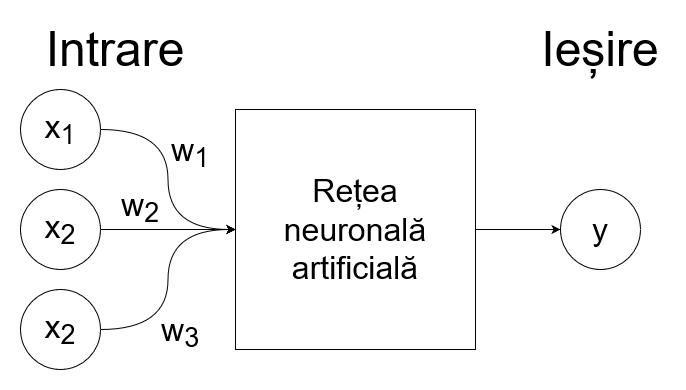
\includegraphics[scale=0.4]{nn_schema_1}
%	\caption{Structura unei re@tele neuronale}
%	\label{nn:schema}
%\end{figure}




\section{Func@tii de activare @si metode de optimizare}
Func@tia de activare ajut@a re@teaua neuronal@a pentru @in@a@tarea de tipare complexe aflate @in setul de date analizat. Alegerea unei func@tii de activare este critic@a pentru performan@ta re@telei, @in special cazul problemelor neliniare.

Unele din cele mai folosite func@tii sunt:

$$
\begin{array}{rlcc}
	{\rm Identitate} & \varphi (x) &=& x \\
	{\rm Binary \, Step} & \varphi (x) &=& \left\lbrace
		\begin{array}{lc}
			1 & x \geq 0 \\
			0 & x < 0
		\end{array}
	\right. \\
	{\rm Logistic, Sigmoid} & \varphi (x) &=& \displaystyle\frac{1}{1 + e^{-x}} \\
	{\rm Rectified\, liniar\, unit (ReLU)}& \varphi (x) &=& \left\lbrace
		\begin{array}{lc}
			x & x \geq 0 \\
			0 & x < 0
		\end{array}
	\right. \\
	{\rm Softplus} & \varphi (x) &=& \ln ( 1 + e^x) \\
\end{array}
$$



\section{Tipuri de re@tele}

De-a lungul anilor, au fost create foarte multe tipuri de re@tele neuronale artificiale pentru a servii la rezolvarea de probleme din domenii dificile.

Exemple de tipuri de re@tele:

\begin{itemize}
	\item Feed Forward (FD)
	\item Deep Feed Forward (DFF)
	\item Radial Basis Network (RBF)
	\item Recurrent Neural Network (RNN)
	\item Long/Short Term Memory (LSTM)
	\item Markov Chain (MC)
	\item Deep Convolutional Network (DCN)
	\item Deconvolutional Network (DN)
	\item Support Vector Machine (SVM)
	\item Deep Belief Network (DBN)
\end{itemize}

%%CAPITOLUL 3
%%
%%
\chapter{Metode de @inv@a@tare}
\index{capitol!C3}

\section{Q-Learning}

%%CAPITOLUL 4
%%
%%
\chapter{Aplica@tie}
\index{capitol!C3}
\section{Structur@a}

Aplica@tia const@a @in antrenarea unor agen@tii care s@a parcurg@a un traseu de curse definit @intr-un mediu 2-dimensional.

Traseul este compus din mai multe sectoare, iar un sector este o por@tiune de drum delimitat@a de dou@a cotituri consecutive.

Fiecare agent poate controla o singur@a sau mai multe ma@sini care s@a participe la completarea traseului. Fiecare ma@sin@a dispune de un numar fix de senzori care ofera agentului detalii despre distan@t@a p\^ n@a la un obiect, tipul obiectului @si sectorul din care face parte.

Aplica@tia este compus@a din 3 par@ti principale:

\begin{itemize}
	\item Simulator - proceseaz@a comenzile agen@tilor @si ofer@a date despre mediul simulat
	\item Interfa@ta grafic@a - permite vizualizarea mediul simulat @si interac@tiunea cu agen@tii
	\item Modele de @inv@a@tare - programe folosite pentru antrenarea agen@tilor prin diferite tehnici folosind datele furnizate de simulator  
\end{itemize}



\section{Simulator}

\section{Interfa@t@a}

\section{Model de @inv@a@tare}

\section{Agent}

%% capitolul de concluzii
%%
%%

\addcontentsline{toc}{chapter}{Concluzii finale}

\markboth{\bf Concluzii finale}{\bf Concluzii finale}

\chapter*{Concluzii finale}

\markboth{\bf Concluzii finale}{\bf Concluzii finale}


\^ In aceast\u a lucrare am analizat ....
\index{concluzii}